\documentclass{article}
\usepackage{ctex}
\usepackage{graphicx}
\usepackage{amsmath}
\usepackage{indentfirst}
\usepackage{titlesec}
\usepackage{setspace}
\usepackage{subfigure}
\usepackage{caption}
\usepackage{float}
\usepackage{booktabs}
\usepackage{geometry}
\usepackage{multirow}
\geometry{left=1.2cm,right=1.2cm,top=2cm,bottom=2cm}
\title{\songti \zihao{2}\bfseries HW2第5题验证Marsaglia抽样方法}
\titleformat*{\section}{\songti\zihao{4}\bfseries}
\titleformat*{\subsection}{\songti\zihao{5}\bfseries}
\renewcommand\thesection{\arabic{section}}
\author{王启骅 PB20020580}
\begin{document}
	\maketitle
	\section{题目}
	对于球面上均匀分布的随机坐标点,给出它们在(x, y)平面上投影的几
	率分布函数。并由此验证Marsaglia抽样方法$ x=2u\sqrt{1-r^2},y=2v\sqrt{1-r^2},z=1-2r^2 $
	确为球面上均匀分布的随机抽样。
	\section{算法原理}
	由于在球面上产生,故取$ \rho=1 $,u,v为两个[-1,1]的均匀分布随机数序列,对于该均匀球面分布有
	\begin{equation}
		dN=\frac{1}{4\pi} sin\theta d\phi d\theta
	\end{equation}
	则可得在xy平面上的投影,面积元变为原来的$ cos\theta $倍,为则分布函数
	\begin{equation}
		\begin{aligned}
			g(x,y)&=2\times \frac{1}{4\pi\times cos\theta}\\
			&=\frac{1}{2\pi\sqrt{1-x^2-y^2}}
		\end{aligned}
	\end{equation}
	
	
	再根据xy与uv的关系式得到
	\begin{equation}
		\begin{vmatrix}
			\frac{\partial x,y}{\partial u,v}
		\end{vmatrix}
	=
	\begin{vmatrix}
		2\sqrt{1-u^2-v^2}-\frac{2u^2}{\sqrt{1-u^2-v^2}}&-\frac{2uv}{1-u^2-v^2}\\
		-\frac{2uv}{1-u^2-v^2}&	2\sqrt{1-u^2-v^2}-\frac{2v^2}{\sqrt{1-u^2-v^2}}
	\end{vmatrix}
=4-8u^2-8v^2
	\end{equation}
	\begin{equation}
		\begin{aligned}
			g(x,y)dxdy&=g(u,v)
				\begin{vmatrix}
				\frac{\partial x,y}{\partial u,v}
			\end{vmatrix}
		dudv\\
		&=\frac{1}{2\pi\sqrt{1-x^2-y^2}}(4-8u^2-8v^2)dudv\\
		&=\frac{2}{\pi}\frac{z}{\sqrt{1-x^2-y^2}}dudv\\
		&=\frac{2}{\pi}dudv
		\end{aligned}
	\end{equation}
\section{结果}
使用Marsaglia抽样方法给出的结果导入到txt文件后用python画图得到球面上的均匀分布点如图
\begin{figure}[!h]
	
	\centering
	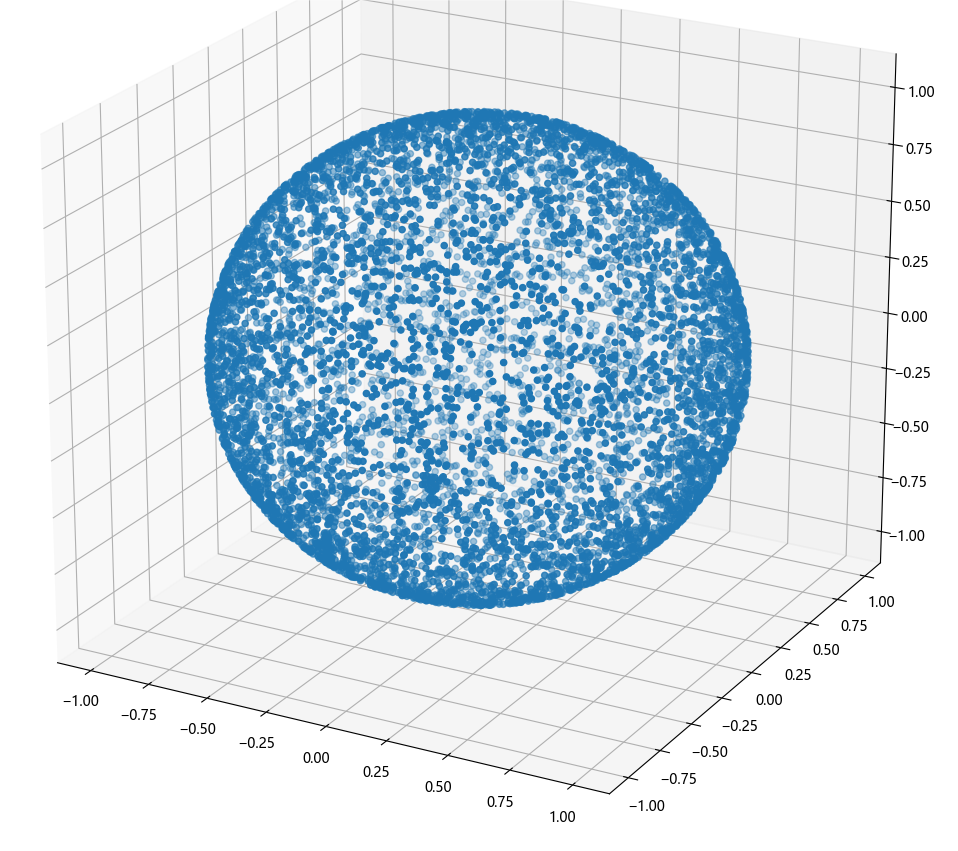
\includegraphics[scale=0.5]{result_2_5}
	\captionsetup{font={small},labelfont=bf}
	\caption{\heiti\zihao{-5}半球面均匀随机分布}
	
\end{figure}
	\section{结论}
	根据u,v的分布函数为常数可得该Marsaglia抽样方法的确为球面上的随机抽样。根据图1可得球面上点是均匀分布的。
\end{document}